\documentclass{article}
\usepackage{parskip}
\usepackage{graphicx}
\usepackage[margin=.6in]{geometry}
\begin{document}
\begin{figure}[htbp]
    \centering
    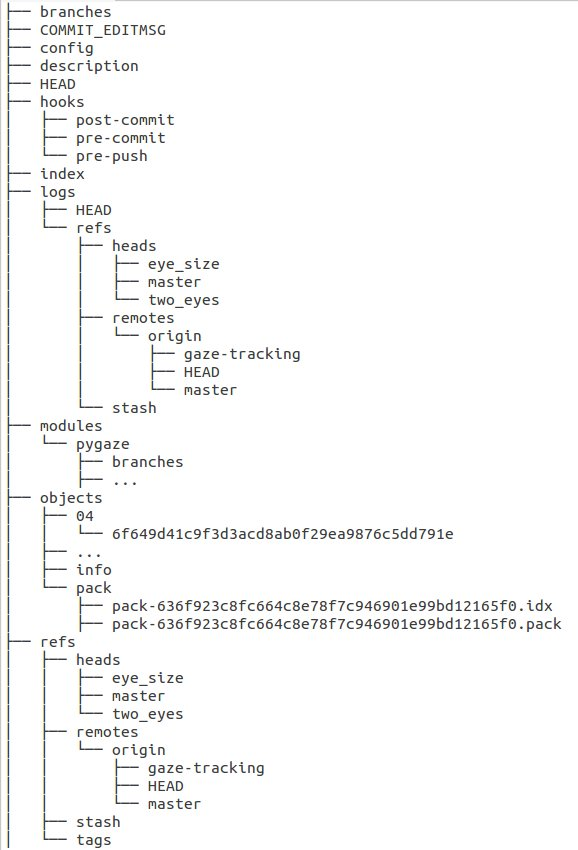
\includegraphics[width=0.5\textwidth]{filestructure.jpeg}
    \caption{Files structure of .git folder}
    \label{fig:file}
\end{figure}

\begin{figure}[htbp]
    \centering
    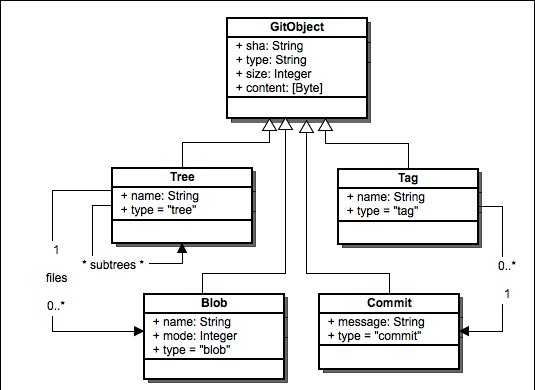
\includegraphics[width=0.95\textwidth]{objects.jpeg}
    \caption{Object hierarchy for git}
    \label{fig:objects}
\end{figure}

\paragraph{File Structure} % (fold)
\label{par:file_structure}
    Figure~\ref{fig:file} displays the file structure of the .git folder for one group members SE390 internal miniproject. The git file structure is broken up into numerous sub folders used to manipulate the git tree. The branches folder contains information needed to manage branches (this is deprecated so the folder is empty). The config folder is contains the git configuration specific to this project. This example did not have any project specific configurations so the folder is empty. Similarly the description folder is empty because it is used to contain information necessary for viewing the repository through a web client an this was not used for this project. The HEAD file stores a reference to which branch you are currently on and the COMMIT\_EDITMSG file stores the last commit message. The hooks folder contains scripts to be executed on triggers defined by its subfolders post-commit, pre-commit, and pre-push. The index is contains information of what changes have been ``added'' and will be committed when the user runs the commit command. This is different from the logs folder which contains all changes that have been made in the history of the repository, the index only contains information that has been added and not committed. The history of the git repository is stored by reference which are heads (referring to the heads of branches the names of which are the subfolders) or remotes (referring to branches that have been pushed). The modules folder outlines submodules that were included. In the example given it is seen as the pygaze module which contains the .git folder for that module so that git knows how to interact with it. The objects folder stores all git objects(the hierarchy of these can be seen in Figure~\ref{fig:objects}) referenced by their sha. Branches are managed by the refs folder which contains references to all local heads (corresponding to all local branchs) and all remote heads (corresponding to all remote branches).
% paragraph file_structure (end)
cite (https://www.siteground.com/tutorials/git/directory.htm)


\paragraph{Object Structure} % (fold)
\label{par:object_structure}
Git manages repositories through a tree of git objects. The UML for this is in Figure~\ref{fig:objects}. All objects are contain a large string called its sha through which you can reference that object. All content in a repository is stored in blob objects and ordered into a tree objects. Each blob represents a file stored in memory. The tree structure represents a directory. Commit objects point at the tree representing the top level directory of the commit. Tags are objects pointing to a single commit for use by the repository history.
% paragraph object_structure (end)
cite(http://aosabook.org/en/git.html).







\end{document}
